% !TEX root = ../Tesis.tex
\chapter{Conclusiones} 
\label{cap:conclusiones} 

Como se mencionó a lo largo del capitulo anterior, se ve en \ref{fig:RMSE} y \ref{fig:MAPE} que los modelos con DWT presentan mayor error, fenómeno que se explica entendiendo que los datos que predice cada una de las redes en las componentes de alta frecuencia agrega ruido a la red y aumenta el error de la reconstrucción. Esto podría sonar a que esta técnica solo ayuda que las redes se equivoquen, pero justamente ayudan a captar la tendencia de la dirección en la que se dirige. Las DWT ha permitido una mejora en la captación de tendencias en los datos a lo largo del tiempo, permitiendo que los modelos produzcan mejores resultados durante más tiempo. Sumado a lo anterior, las redes recurrentes superaron ampliamente a la red auto-regresiva, ya que durante todo el capitulo anterior mostraron tanto menor error en la predicción de valores como de dirección.

A lo largo del entrenamiento, se pudo comprobar que como bien señala Prudhviraju Srivatsavaya \cite{GRU_vs_LSTM}, gracias a que los parámetros y complejidad en una LSTMnn son mayores que en una GRUnn, el tiempo de entrenamiento es lógicamente mayor, hecho que suma un punto a favor de esta arquitectura. Con este análisis, podemos decir que el mejor paradigma fue el recurrente, empleando la DWT sobre la GRUnn.

%Sin embargo, no olvidemos que la predicción de precios de instrumentos financieros a lo largo del tiempo conlleva un reto importante y es vital no mantenerse atados a una sola tecnología cuando realizamos una investigación de este tipo. Existe una cantidad abismal de herramientas y técnicas que nos acercan cada día más a nuestros objetivos. Además de la creciente demanda de procesamiento de datos no dejemos de lado el análisis de otras variables sociales, políticas y culturales que impactan en estos estudios. Es por esta razón que este estudio no representa un cierre a la temática, si no que podemos encontrar en herramientas como la atención o modelos como los transformadores, buenos temas para continuar la investigación a futuro.

\subsection{Investigación a Futuro}

A partir de este punto, en futuras investigaciones, es importante explorar otros enfoques avanzados que han demostrado ser efectivos en la predicción de series de tiempo y precios de acciones. Modelos como las redes neuronales de atención y los transformadores (\textit{Transformer Networks}), que ya han sido revolucionarios en procesamiento de lenguaje natural, están ganando terreno en el análisis de secuencias financieras debido a su capacidad para captar dependencias a largo plazo y patrones más complejos. Además, se puede investigar la implementación de técnicas de aprendizaje por refuerzo (\textit{reinforcement learning}) para el desarrollo de estrategias para operaciones bursátiles adaptativas.

Asimismo, sería relevante integrar enfoques multimodales, combinando no solo datos históricos de precios, sino también variables ajenas a las matemáticas, como eventos políticos, cambios regulatorios, indicadores económicos, y análisis de sentimiento a partir de noticias o redes sociales. Estas variables externas pueden mejorar la capacidad de los modelos para predecir movimientos del mercado.

Finalmente, el uso de redes neuronales más avanzadas, como las Redes Neuronales Gráficas \textit{Graph Neural Networks} (GNNs) \cite{graphNN} para capturar las relaciones entre diferentes activos financieros también se presentan como prometedoras para futuras investigaciones. Esto permitiría desarrollar modelos que sean más robustos ante la volatilidad y que puedan adaptarse mejor a las condiciones cambiantes del mercado financiero.

\subsection{Proyecto a Futuro}

Como parte del trabajo a futuro y de la integración de este estudio a un proyecto de análisis financiero, se puede pensar en un servicio que combine una plataforma similar a la terminal de \textit{Bloomberg} con predicción de series de tiempo. Este podría ofrecer una herramienta poderosa para la extrapolación de precios de emisoras en mercados financieros que permitiera a inversionistas particulares información valiosa sobre sus compras.

\begin{figure}[H]
    \centering
    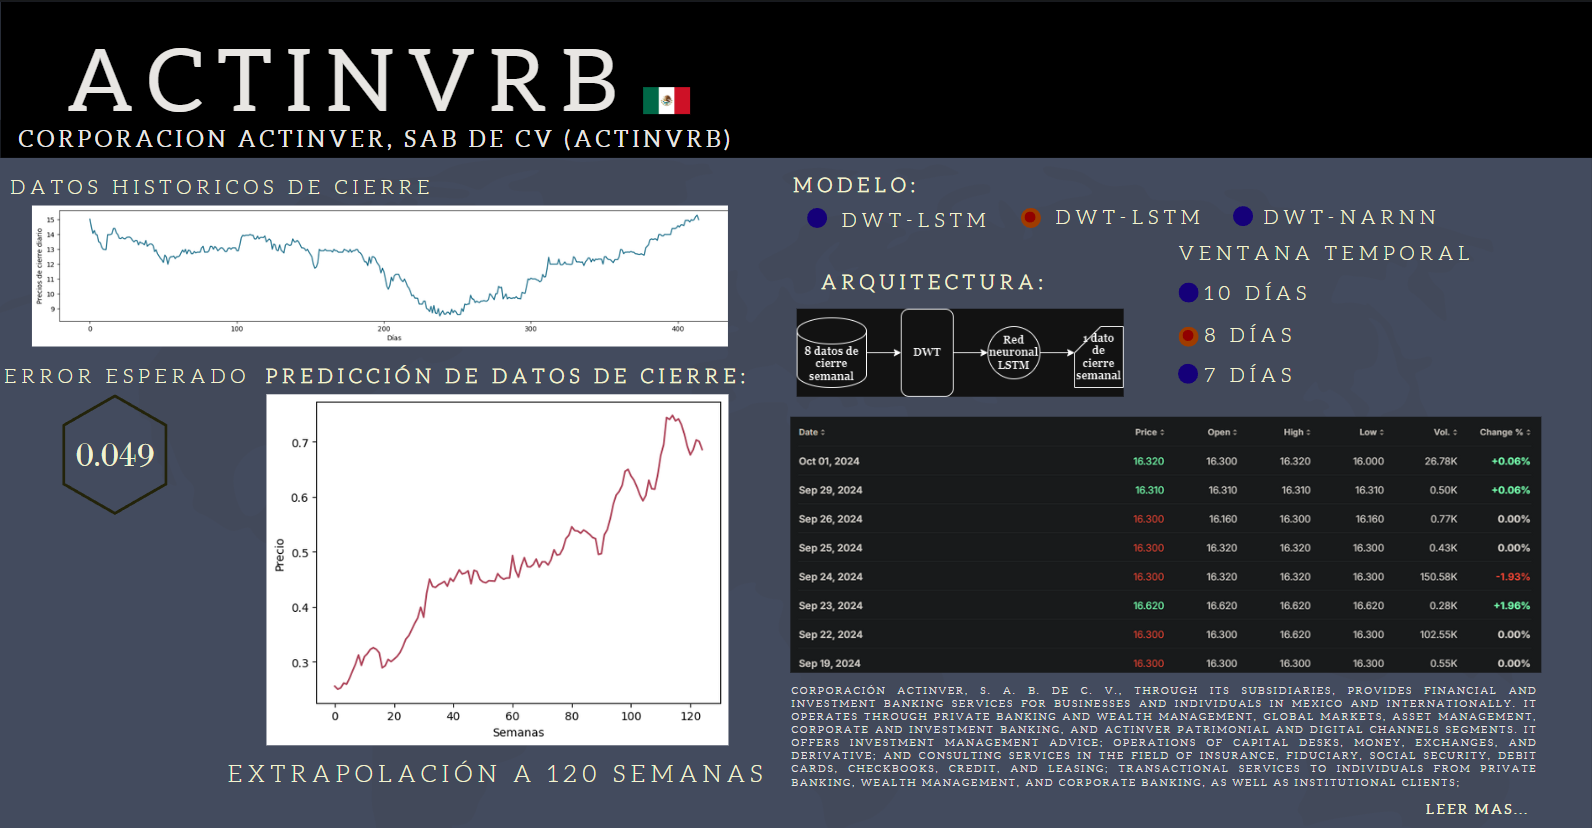
\includegraphics[width=1\textwidth]{Figuras/conclusiones/modelo_app.png}
    \caption{Bosquejo de ventana para predicción de datos.} 
    \label{fig:aplicacion}
\end{figure}

Una plataforma que permite a los usuarios acceder a datos financieros históricos y en tiempo real, y realizar predicciones sobre precios futuros de acciones, bonos u otros activos financieros utilizando no solo redes neuronales, sino otras técnicas que mencionadas en la sección anterior. Podría incluir:

\begin{enumerate}
    \item Acceso a predicciones personalizadas: Los usuarios podrían seleccionar emisoras específicas para recibir predicciones a corto y largo plazo basadas en los datos históricos.
    \item Visualización interactiva: Gráficos interactivos que muestran tanto datos históricos como predicciones futuras, con intervalos de confianza y métricas de precisión.
    \item Alertas y notificaciones: Los usuarios recibirían alertas cuando se predigan fluctuaciones importantes en los precios de activos.
\end{enumerate}

La fuente de los datos financieros partiría del consumo de datos de precios en tiempo real y datos históricos de varias fuentes confiables. En ese sentido, se valdría de:

\begin{enumerate}
    \item APIs de Datos Financieros: El servicio podría consumir datos desde APIs con un enfoque en obtener precios históricos, volumen, datos de mercado y otros indicadores financieros.
    \item Procesamiento y Limpieza de Datos: Una vez que los datos se obtienen de las APIs, serían preprocesados para eliminar valores faltantes, detectar anomalías y preparar los conjuntos de datos para ser usados por los modelos de predicción. Esto podría incluir transformaciones como la descomposición de series temporales.
\end{enumerate}

%3. Arquitectura del Servicio
Además, El servicio podría estar basado en una arquitectura distribuida, combinando varios componentes para manejar las predicciones en tiempo real y permitir la escalabilidad.

%a. Backend de Datos
%Este componente manejaría la recopilación y almacenamiento de los datos financieros. Podría incluir:

%Bases de datos relacionales (SQL): Para almacenar datos estructurados como precios históricos, información de las emisoras, o variables macroeconómicas.
%Bases de datos NoSQL (MongoDB, Cassandra): Para almacenar grandes volúmenes de datos no estructurados o semi-estructurados, como registros de transacciones en tiempo real.
%b. Módulo de Predicción
%El núcleo del sistema de predicción estaría compuesto por modelos de redes neuronales especializadas, como:

%LSTM (Long Short-Term Memory) y GRU: Estas son arquitecturas recurrentes adecuadas para la predicción de series de tiempo, debido a su capacidad para capturar patrones a largo plazo.
%Modelos Híbridos (CNN-LSTM, Transformers): Para mejorar la precisión, podrían implementarse arquitecturas híbridas que combinen convoluciones y recurrencias para capturar tanto patrones locales como globales.
%El servicio permitiría a los usuarios realizar predicciones de diferentes tipos:

El enfoque principal del pronostico con los modelos serían las predicciones a corto plazo con horizontes temporales de días o semanas. Sumadas a las predicciones basadas en patrones estacionales o tendencias a largo plazo.
%c. API REST para la Comunicación
%La aplicación podría utilizar una API REST para permitir que los usuarios y otros sistemas interactúen con el servicio de predicción. Esta API podría exponer varias funcionalidades, como:

%Solicitar predicciones para una emisora.
%Obtener datos históricos y en tiempo real.
%Visualizar gráficos de precios proyectados.
%d. Frontend de Usuario
%El frontend del sistema sería una interfaz web accesible a través de navegadores o aplicaciones móviles. El diseño debe ser intuitivo, con herramientas de visualización como:

%Gráficos de líneas y velas: Para mostrar precios históricos y predicciones.
%Panel de control personalizable: Para que los usuarios puedan gestionar sus emisoras favoritas y ver las predicciones relevantes.
%Señales y alertas: Donde el usuario pueda recibir notificaciones basadas en predicciones o eventos relevantes.
%e. Infraestructura en la Nube
%El servicio podría ser desplegado en la nube (AWS, Google Cloud, Microsoft Azure), lo que permitiría escalabilidad, alta disponibilidad y la capacidad de procesar grandes volúmenes de datos en tiempo real. Los modelos de predicción podrían ser servidos a través de microservicios, lo que permitiría una integración flexible y un despliegue continuo.

%4. Entrenamiento y Validación de Modelos
%El proceso de entrenamiento de los modelos implicaría:

%Entrenamiento con datos históricos: Los modelos serían entrenados con grandes volúmenes de datos históricos de precios de las emisoras y otros indicadores financieros (volumen, noticias económicas, etc.).
%Validación cruzada y prueba de modelos: Se usarían técnicas como la validación cruzada para evitar sobreajuste y garantizar que los modelos sean robustos y precisos.
%Ajuste de hiperparámetros: Se podrían emplear técnicas como la búsqueda en cuadrícula o el ajuste bayesiano para optimizar los hiperparámetros de los modelos.
%5. Organización del Desarrollo
%El desarrollo de un servicio de este tipo implicaría una organización clara de los equipos y las tareas:

%Equipo de Ingeniería de Datos: Encargado de la recopilación, limpieza y procesamiento de datos financieros.
%Equipo de Científicos de Datos: Responsable de diseñar, entrenar y ajustar los modelos de redes neuronales para la predicción.
%Equipo de Backend y APIs: Encargado de implementar la arquitectura del sistema, integrando la API REST y los microservicios necesarios.
%Equipo de DevOps: Para gestionar el despliegue, la escalabilidad y la infraestructura en la nube.
%Equipo de Frontend: Responsable de desarrollar la interfaz de usuario y las herramientas de visualización.
%6. Monetización y Escalabilidad
%Este servicio podría monetizarse a través de suscripciones, donde los usuarios paguen por acceso a predicciones premium, más detalladas o con mayor frecuencia de actualización. También podría ofrecerse como una API para empresas interesadas en incorporar predicciones a sus propios sistemas.

En cuanto a la escalabilidad, los modelos de predicción deben actualizarse constantemente con nuevos datos, lo que necesitaría de un sistema robusto para gestionar grandes cantidades de información y realizar inferencias rápidas en tiempo real.

Este servicio ofrecería un enfoque nuevo para análisis financiero, combinando datos en tiempo real con técnicas avanzadas de predicción de series de tiempo para mejorar la precisión de las predicciones en mercados volátiles, con una arquitectura flexible y escalable en la nube. 